En comparación con LAMP, el paquete de aplicaciones MEAN es bastante nuevo. Una de sus mayores diferencias es que MEAN no depende de un sistema operativo específico. Node.js se encarga de la ejecución del lado del servidor. MEAN Stack se recomienda especialmente para desarrolladores de JavaScript, ya que utiliza JavaScript en todos los niveles, tanto para el código del lado del cliente, así como el código del lado del servidor \cite{srinivasan}.
\vspace{0.8cm}

\subsection{Componentes MEAN}
\begin{itemize}
  \item MongoDB (base de datos)\\
  Una opción increíblemente popular en el mundo de la gestión de bases de datos NoSQL.
  \item Express.js (servidor)\\
  Para manejar las solicitudes de enrutamiento y proporcionar una API REST, o incluso puede usarse para generar el HTML final para ser utilizado por el framework de \textit{frontend}.
  \item Angular.js / React.js (cliente)\\
  Es un potente framework \textit{frontend}, utiliza un patrón de diseño Modelo-Vista-Controlador. React.js es una opción alternativa para el desarrollo \textit{frontend}, aunque React es simplemente una biblioteca, no un framework MVC completo.
  \item Node.js (entorno del servidor)\\
  Permite al programador escribir el \textit{backend} de la aplicación en Javascript y ejecutarlo en la mayoría de los sistemas operativos modernos.
\end{itemize}

Derivados:

\begin{itemize}
  \item MERN (React.js en lugar de Angular.js)
  \item MEEN (Ember.js en lugar de Angular.js)
\end{itemize} 

\begin{figure}[H]
  \centering
  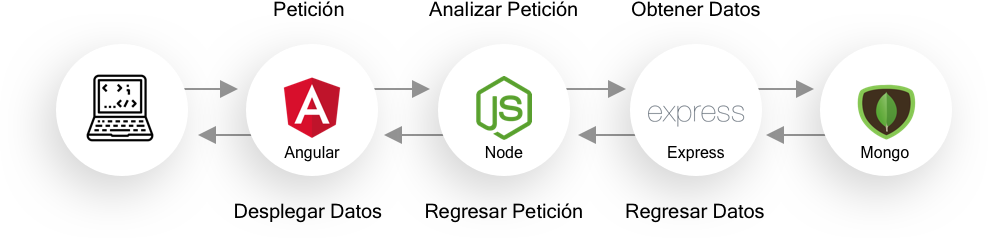
\includegraphics[width=1\textwidth]{mean}
  \caption{Flujo de información en MEAN Stack.}
\end{figure}

\subsection{Beneficios}
Usar JavaScript como el lenguaje de programación principal es una gran ventaja. Todo se puede configurar rápidamente y hacer en JavaScript, lo que hace que sea mucho más fácil encontrar desarrolladores, y los desarrolladores de LAMP generalmente también conocen JavaScript. Otra gran ventaja es la capacidad de crear fácilmente aplicaciones móviles o de escritorio, por ejemplo con Ionic. El código y los componentes se pueden reutilizar o agregar fácilmente.

\subsection{Desventajas}
Muchas librerías y \textit{frameworks} son bastante nuevos, y las nuevas versiones se lanzan rápidamente, por lo que mantener una aplicación puede ser una molestia. Dado que muchas tecnologías desaparecen después de unos años, la sostenibilidad puede convertirse en un problema. También es más difícil mantener una base de código limpia y seguir las mejores prácticas a medida que su aplicación crece. Además, debe confiar en el cliente y las tecnologías disponibles del cliente.

\newpage
\subsection{Base de datos NoSQL}
A pesar de la gran cantidad de bases de datos SQL, también hay una tendencia hacia NoSQL. Las bases de datos NoSQL permiten almacenar datos no estructurados y heterogéneos. La escalabilidad mejorada ha ayudado a aumentar su popularidad en mayor medida en el mercado actual. El escalado horizontal significa que la organización no tiene que preocuparse por la infraestructura subyacente. Las bases de datos NoSQL son una alternativa emergente a las bases de datos relacionales más utilizadas. Como su nombre lo indica, no reemplaza completamente a SQL, sino que lo complementa de tal manera que puedan coexistir.
\vspace{0.8cm}

\begin{table}[H]
  \renewcommand{\arraystretch}{1.5}
  \centering
  \scriptsize
  \begin{tabular}{ |p{2cm}||p{5cm}|p{5cm}|  }
    \hline
      & SQL
      & NoSQL \\
    \hline
    Tipo
      & Relacional
      & Distribuido \\
    \hline
    Datos
      & Datos estructurados almacenados en tablas 
      & Datos no estructurados almacenados en archivos JSON \\
    \hline
    Esquema 
      & Estático o predefinido
      & Dinámico \\
    \hline
    Escalable 
      & Vertical
      & Horizontal \\
    \hline
    Consultas
      & Adecuado para consultas complejas 
      & Lenguaje de consulta no estructurado \\
    \hline
    Flexible
      & Esquema rígido ligado a la relación 
      & Esquema adecuado para almacenamiento jerárquico \\
    \hline
    Elasticidad
      & Requiere tiempo de inactividad en la mayoría de los casos 
      & Automática, no requiere interrupción \\
    \hline
  \end{tabular}
  \caption{Comparativa SQL y NoSQL}
\end{table}
\vspace{0.8cm}

El concepto de NoSQL se desarrolló hace mucho tiempo, pero fue después de la introducción de la base de datos como servicio (DBaaS) que obtuvo un reconocimiento destacado. Debido a la alta escalabilidad proporcionada por NoSQL, fue visto como un importante competidor del modelo de base de datos relacional. A diferencia de las bases de datos relacionales (RDB), las bases de datos NoSQL están diseñadas para escalar fácilmente a medida que crecen. La mayoría de los sistemas NoSQL han eliminado el soporte multiplataforma y algunas características adicionales innecesarias de RDBMS, haciéndolos mucho más livianos y eficientes que sus contrapartes RDMS.


\subsection{Orientado a documentos}
El concepto principal de una base de datos orientada a documentos es que el documento contiene grandes cantidades de datos que pueden estar disponibles de manera útil. Se puede acceder a estos documentos como un directorio regular en el que puede tener diferentes colecciones y cada colección tiene documentos que contienen la información deseada. Además, cada colección puede tener colecciones internas. Puede tener un árbol completo de documentos, sin embargo, esta práctica no se recomienda y debe evitar tener más de tres niveles de anidamiento. 
\vspace{0.8cm}

Las bases de datos NoSQL no son necesariamente bases de datos relacionales. Los datos no son representados en términos de filas y columnas de tablas. En MongoDB, los datos se visualizan como objetos o documentos. Esto ayuda a un programador a evitar una capa de traducción, por lo que no es necesario convertir o asignar los objetos con los que trata el código en tablas relacionales. Dichas traducciones se denominan capas de Mapeo Relacional de Objetos (ORM).
\begin{figure}[H]
  \centering
  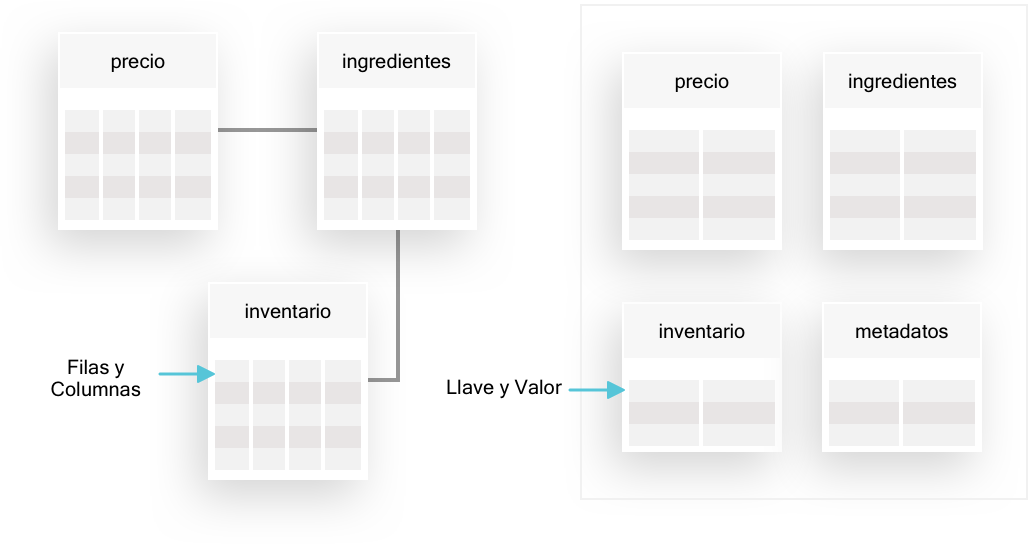
\includegraphics[width=1\textwidth]{sql-nosql}
  \caption{Diagrama que representa las diferencias clave entre la base de datos SQL y las bases de datos NoSQL.}
\end{figure}

\subsection{Angular/React}
Angular o React, proporcionan la interfaz de usuario reactiva de una aplicación. Utilizan componentes, son reactivos porque el usuario recibe cambios inmediatos cuando interactúa con la aplicación y, por lo general, se ejecutan dentro del navegador de un usuario (aunque ambos son isomórficos, capaces de ejecutarse en un servidor).
\vspace{0.8cm}

\begin{table}[H]
  \renewcommand{\arraystretch}{1.5}
  \centering
  \scriptsize
  \begin{tabular}{ |p{2cm}||p{5cm}|p{5cm}|  }
    \hline
      & Angular
      & React \\
    \hline
    Desarrollador
      & Google
      & Facebook \\
    \hline
    Definición
      & Framework
      & Librería \\
    \hline
    Modelo de plantilla
      & HTML + Typescript
      & JSX + Javascript \\
    \hline
    Flujo
      & 2 vías
      & Unidireccional \\
    \hline
    DOM
      & Regular
      & Virtual \\
    \hline
    Lógica/Estado de la aplicación
      & Services
      & Flux/Redux \\
    \hline
  \end{tabular}
  \caption{Características de Angular.js y React.js}
\end{table}
\vspace{0.8cm}

Angular es un framework con muchas herramientas integradas, para hacer solicitudes HTTP, enrutamiento y navegación, animaciones y otros. Se basa en módulos que son componentes y servicios.
\vspace{0.8cm}

React es una biblioteca de Javascript, que se puede usar para crear nuevas aplicaciones o para integrarla con una aplicación existente. React se basa en componentes pequeños y reutilizables, que administran su propio estado y luego los componen para crear interfaces de usuario complejas. Incluso si React no es tan complejo como Angular, con muchas cosas integradas, hay muchas bibliotecas que se pueden agregar para tener enrutadores (react-router) y solicitudes HTTP (axios), manejo de estado (react-redux) entre otras más. Esto lo hace portátil y fácil de incorporar en cualquier entorno.